
\goodbreak
\newpage
\clearpage

\section[CMAC]{CMAC}
\label{cmac_sec}

A \emph{Cerebellar Model Articulation Controller} (CMAC) foi criada por James Sacra Albus \cite{Albus1975b}. 
Ele se inspirou no cerebelo dos mamíferos para criá-la. 
O mesmo autor havia feito um extenso trabalho sobre o funcionamento do cerebelo \cite{Albus1971b}.
Trabalho este, que resultou numa tese de doutorado \cite{Albus1972a}.
Aplicações da CMAC podem ser vistas em \cite{Albus1975d}, \cite{Albus1979}, \cite{Sabourin2006a} e \cite{Lin2002a}.
Uma aplicação que começou a ser desenvolvida pela UnB é descrita em \citeonline{Andrade2014}. Inclusive a implementação da \emph{CMAC} desenvolvida neste trabalho teve origem nele.

Na Figura \ref{fig1} é possível ver o funcionamento básico da CMAC. Os sinais $S$ entram no sistema, que mapeiam o mesmo para um conjunto de pesos $W^*$ que devem ser somados para ativação. 
Note que apenas uma pequena fração de pesos é realmente selecionada para participar na ativação. 
O conjunto de pesos disponíveis na CMAC é necessariamente maior que o número de pesos ativados $W^*$. 

A CMAC da Figura \ref{fig1} também pode ser classificada como um sistema \emph{Multiple Input Single Output} (MISO), ou seja, suporta a entrada de vários sinais de entrada e processa um sinal de saída.
Para se produzir uma CMAC \emph{Multiple Input Multiple Output} MIMO, bastaria implementar várias MISOs, compartilhando as mesmas entradas.


Os passos para que o sinal seja computado são descritos a seguir. Estes passos são os mesmos descritos em \citeonline{Albus1975b}.

Primeiramente, define-se o número de pesos $NW*$ a serem ativados para comporem a saída da CMAC.

O segundo passo é quantizar os possíveis valores para cada item do vetor de entrada $S$.
Por exemplo, se o primeiro item $s1$ de $S$ aceita valores de -1 até 1 e se quer 5 valores possíveis, quantiza-se então os valores de -1 até 1, conforme Figura \ref{inputs1}.



Isto significa que quaisquer que sejam os valores de $s1$ os mesmos devem ser convertidos para -1, -0,5, 0, 0,5 e 1. 
Por exemplo, se o valor de $s1$ for 0,75, será convertido para o valor 1, se for -0,75 será o valor 0 e se for 0,25 será o valor 0,5. A esta quantização dá-se o nome de resolução da CMAC \cite{Albus1975b}.

O próximo passo é criar uma tabela para cada um dos sinais discretizados de entrada do vetor $S$. 
Supondo que o vetor $S$ possui 2 sinais de entrada $s1$ e $s2$ e um número de ativações $NW*$ igual a 3, deve-se criar duas tabelas, uma para cada sinal, conforme se apresentam na Tabela \ref{disc_s1} e na Tabela \ref{disc_s2}. 
Para facilitar o entendimento, irá se considerar os valores possíveis de $s1$ iguais aos inteiros de 1 até 6 e os valores possíveis de $s2$ iguais aos inteiros de 1 até 4.
Cria-se uma coluna com os valores do sinal em questão. 
Para cada valor, cria-se 3 ($NW*$) valores novos. 
Para o primeiro valor do sinal, usa-se os 3 primeiros inteiros não negativos.
Para o segundo valor do sinal, substitui-se o primeiro dos três itens pelo próximo número após o terceiro item do sinal anterior. 
Para o terceiro sinal, substitui-se o segundo dos três itens pelo próximo inteiro não negativo.
Assim, sucessivamente conforme a Tabela \ref{disc_s1} e Tabela \ref{disc_s2} \cite{Albus1975b}.

\begin{figure}[ht]
	\centering
	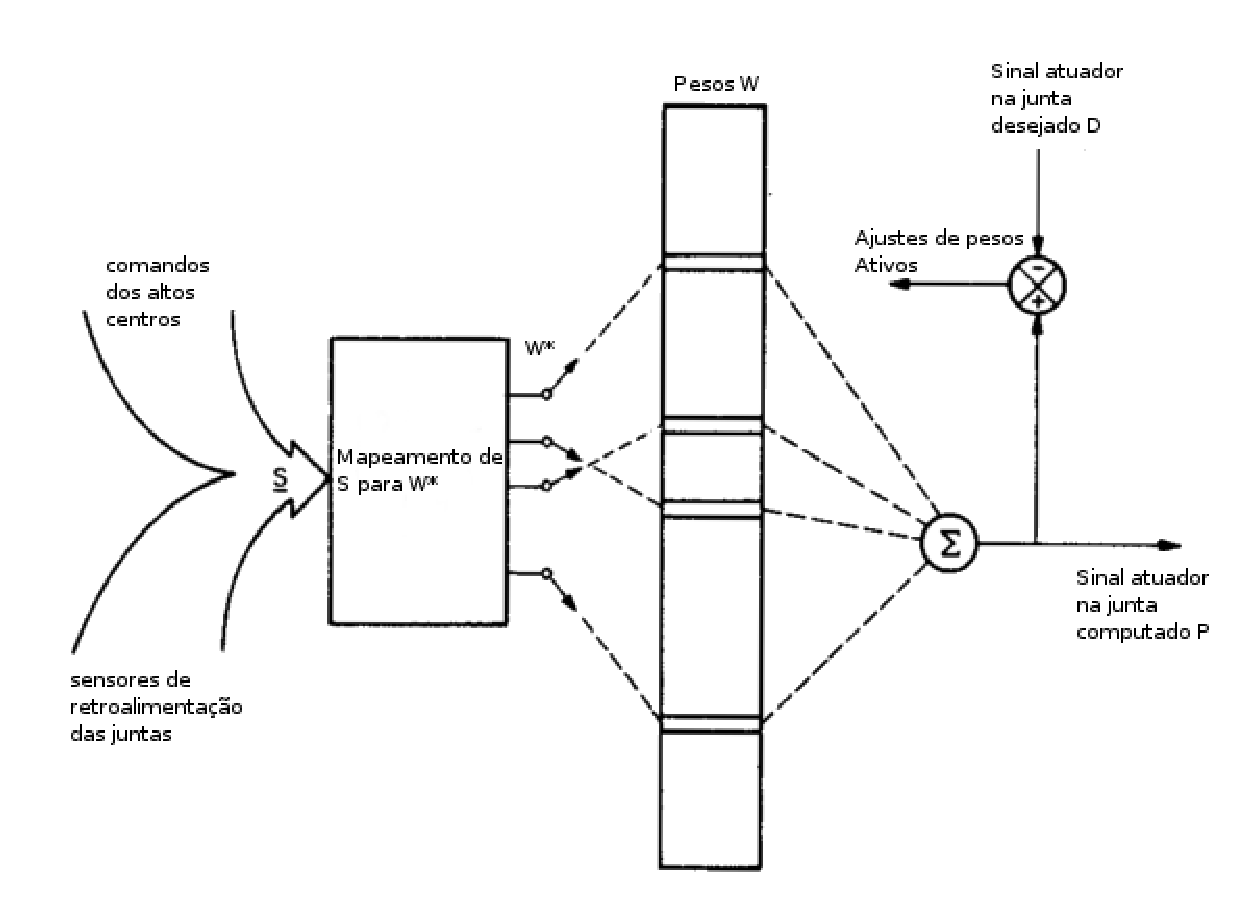
\includegraphics[width=15 cm]{figuras/cmac1.eps}
	\caption{CMAC para controle de uma junta. Adaptado de \cite{Albus1975b}.}
    	\label{fig1}
\end{figure}


\begin{figure}[ht]
	\centering
	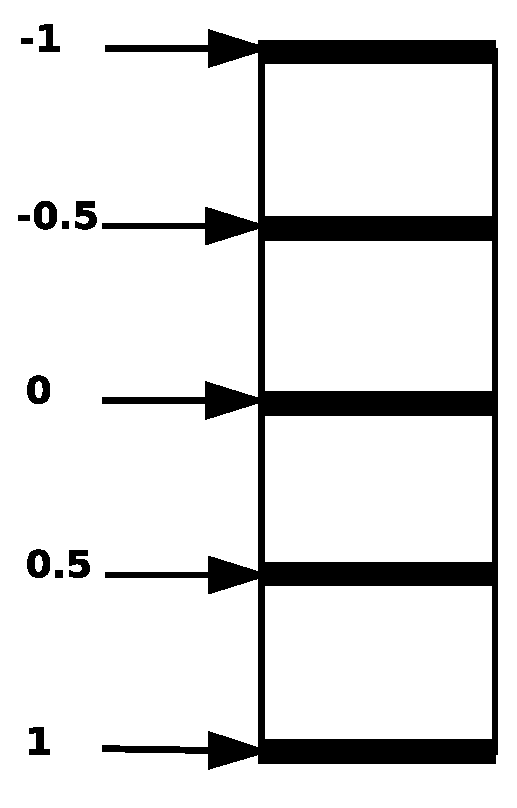
\includegraphics[width=3 cm]{figuras/input.eps}
	\caption{Quantização de $s1$.}
    	\label{inputs1}
\end{figure}

\begin{table}[ht]
	\centering
	\caption{Mapeamento de $s1$}
	\label{disc_s1}
	\ABNTEXfontereduzida
	\begin{tabular}{c c}
		\toprule
		\textit{Valore de $s1$} & \textit{Mapeamento $m1$}\\
		\midrule
		\ABNTEXfontereduzida
		1 & 0, 1, 2 \\
		2 & 3, 1, 2 \\
		3 & 3, 4, 2 \\
		4 & 3, 4, 5 \\
		5 & 6, 4, 5 \\
		6 & 6, 7, 5 \\
		\bottomrule
	\end{tabular}
\end{table}
\begin{table}[ht]
	\centering
	\caption{Mapeamento de $s2$}
	\label{disc_s2}
	\ABNTEXfontereduzida
	\begin{tabular}{c c}
		\toprule
		\textit{Valore de $s2$} & \textit{Mapeamento $m2$}\\
		\midrule
		\ABNTEXfontereduzida
		1 & 0, 1, 2 \\
		2 & 3, 1, 2 \\
		3 & 3, 4, 2 \\
		4 & 3, 4, 5 \\
		\bottomrule
	\end{tabular}
\end{table}


Depois de mapeado cada valor de cada item de entrada, deve-se combinar os mapeamentos de acordo com a Tabela \ref{wmap}.

O mapeamento da Tabela \ref{wmap} é feito da seguinte forma \cite{Albus1975b}: 
Coloca-se cada valor quantizado de $s1$ nomeando cada uma das linhas da tabela. 
Coloca-se cada valor discretizado de $s2$ nomeando cada uma das colunas das tabelas. 
Cada célula da tabela é obtida recuperando-se os itens de $s1$ e de $s2$, que estão na Tabela \ref{disc_s1} e na Tabela \ref{disc_s2}, e concatenando-se cada item de acordo com sua posição. 
Por exemplo, para o valor de $s1$ igual a 5, recuperam-se os itens (6, 4, 5), para o valor de $s2$ igual a 2, recuperam-se os itens (3, 1, 2). 
Agora é só criar novos itens, na mesma quantidade do valor $NW*$, concatenando-se cada item de acordo com sua posição. O lista resultante é ((6, 3), (4, 1), (5, 2)). 

Cada vetor de 2 posições da Tabela \ref{wmap}, por exemplo (0, 0), (4, 1), é um rótulo de uma entrada na tabela de pesos $W$.

Para se calcular a saída do sistema, suponha que os valores de $s1$ e $s2$, ainda sejam 5 e 2, respectivamente, e $NW*$ ainda seja 3. 
Neste caso, recupera-se o item da linha 5 e da coluna 2, que é ((6, 3), (4, 1), (5, 2)). 
Agora é acessada a tabela de pesos W e são recuperados os pesos cujas chaves são (6, 3), (4, 1) e (5, 2). 
Note-se que serão recuperados exatamente 3 pesos, que é exatamente o número de ativações $NW*$ desejadas. 
Os valores recuperados constituem um vetor chamado $W*$. A saída é calculada somando-se os valores de W*.



\begin{table}[ht]
	\centering
	\caption{Mapeamento para os pesos $W$}
	\label{wmap}
	\ABNTEXfontereduzida
	\begin{tabular}{c c c c c}
		\toprule
		\textit{$s1$ / $s2$} & \textit{1}  & \textit{2} & \textit{3} & \textit{4} \\
		\midrule
		\ABNTEXfontereduzida

		\textit{1} & (0, 0), (1, 1), (2, 2) & (0, 3), (1, 1), (2, 2) & (0, 3), (1, 4), (2, 2) & (0, 3), (1, 4), (2, 5) \\
		\textit{2} & (3, 0), (1, 1), (2, 2) & (3, 3), (1, 1), (2, 2) & (3, 3), (1, 4), (2, 2) & (3, 3), (1, 4), (2, 5) \\
		\textit{3} & (3, 0), (4, 1), (2, 2) & (3, 3), (4, 1), (2, 2) & (3, 3), (4, 4), (2, 2) & (3, 3), (4, 4), (2, 5) \\
		\textit{4} & (3, 0), (4, 1), (5, 2) & (3, 3), (4, 1), (5, 2) & (3, 3), (4, 4), (5, 2) & (3, 3), (4, 4), (5, 5) \\
		\textit{5} & (6, 0), (4, 1), (5, 2) & (6, 3), (4, 1), (5, 2) & (6, 3), (4, 4), (5, 2) & (6, 3), (4, 4), (5, 5) \\
		\textit{6} & (6, 0), (7, 1), (5, 2) & (6, 3), (7, 1), (5, 2) & (6, 3), (7, 4), (5, 2) & (6, 3), (7, 4), (5, 5) \\

		\bottomrule
	\end{tabular}
\end{table}
 


\subsection{TREINAMENTO DA CMAC}
Sendo a CMAC uma Rede Neural Artificial (RNA) com aprendizado supervisionado, seus pesos podem ser atualizados simplesmente computando-se o erro e atualizando-se apenas os pesos que participaram do computo do sinal $P$ \cite{Haykin1998}. O processo é detalhado nos próximos parágrafos.

Para se treinar a CMAC, primeiro define-se o conjunto de dados para treinamento que devem ser usados. 
Pode ser usado algo entre 20\% e 50\% dos dados coletados para desenvolvimento do sistema. 
Cada item destes dados deve conter um vetor de sinais de entradas $S$ e a resposta desejada $D$ para estes sinais. 
A tabela de pesos deve ser inicializada com valores randômicos. 
Para cada vetor $S$ deve ser calculado o vetor $W*$, que contém os endereços dos pesos a serem ativados. 
Calcula-se, então, a saída da rede $P$ para o vetor $S$, conforme definido no item \ref{cmac_sec}, somando os itens do vetor $W$. 
Atualizam-se os pesos sinápticos conforme a Equação \ref{write_weight} adaptada de \citeonline{Sabourin2012a}.
\begin{equation}
	\label{write_weight}
	w_{i} = w_{i} + \cfrac{\alpha (D - P)}{NW^{*}}
\end{equation}

A variável $w_{i}$ é um item qualquer dentro da tabela de pesos $W$. 
Em cada iteração no conjunto de dados para treinamento, deve-se atualizar apenas os pesos descritos em $W*$ naquele momento. 
A variável $\alpha$ é o coeficiente de aprendizado, deve ser um valor entre 0 e 1. 
A variável $NW*$ é o número de valores a serem utilizados para ativação, que consequentemente equivale ao número de itens do vetor $W*$.

Deve-se determinar o número de iterações \emph{batch} para o sistema. 
Uma iteração \emph{batch} consiste no processamento dos pesos para cada item dentro do conjunto de dados para treinamento \cite{Ng2015}. 
O sistema deve continuar iterando até atingir o número de iterações \emph{batch}.

Apesar do número de iterações \emph{batch} ser válido como critério de parada para o treinamento da CMAC, nada impede o uso de outros critérios, por exemplo, o erro quadrado médio da saída $Y$ em relação ao desejado $D$.
